% CGO 09: http://www.cgo.org/
% svn co https://svn.mcs.anl.gov/repos/performance/orio/doc/papers/cgo08
% Max 22 pages, double-spaced, 11pt or larger font
% Abstract 300 words: Sep. 12, 2008
% Full paper: Sep. 19, 2008

\documentclass[runningheads]{llncs}

\usepackage{amssymb}
\setcounter{tocdepth}{3}
\usepackage{graphicx}
\usepackage{url}
\usepackage{html}
\usepackage{setspace}
\usepackage{graphicx}
\usepackage{subfigure}
\usepackage{cite}
\usepackage{amsmath}

\urldef{\mailsa}\path|{alfred.hofmann,ursula.barth,ingrid.beyer,natalie.brecht,|
\urldef{\mailsb}\path|christine.guenther,frank.holzwarth,piamaria.karbach,|
\urldef{\mailsc}\path|anna.kramer,erika.siebert-cole,lncs}@springer.com|
\newcommand{\keywords}[1]{\par\addvspace\baselineskip
\noindent\keywordname\enspace\ignorespaces#1}

\newenvironment{itemizer}{\begin{itemize}\setlength{\parsep}{0cm}\setlength{\itemsep}{-.3em}}{\end{itemize}}

\begin{document}

\mainmatter  % start of an individual contribution

% first the title is needed
\title{Generating Empirically Optimized Numerical Software from MATLAB Prototypes}

        % a short form should be given in case it is too long for the running head
        \titlerunning{Empiriclaly Optimized Numerical Software from MATLAB}

        % the name(s) of the author(s) follow(s) next
        %
        % NB: Chinese authors should write their first names(s) in front of
        % their surnames. This ensures that the names appear correctly in
        % the running heads and the author index.
        %
\author{Elizabeth Jessup\inst{1} 
  \and Boyana Norris\inst{2}
  \and Albert Hartono\inst{3}
  \and Jeremy Siek\inst{1}}

\authorrunning{Jessup, Norris, Hartono, Siek}

\institute{University of Colorado at Boulder \\
  \email{\{elisabeth.jessup,jeremy.siek\}@colorado.edu}
  \and Argonne National Laboratory \\
  \email{\{norris\}@mcs.anl.gov}
  \and Ohio State University \\
  \email{\{hartonoa\}@cse.ohio-state.edu}}

%\toctitle{Lecture Notes in Computer Science}
\tocauthor{Elizabeth Jessup, Boyana Norris, Albert Hartono, and Jeremy Siek}
\maketitle

\begin{abstract}
% between 75 and 150 words
The growing demand for higher levels of detail and accuracy in results means that the size and complexity of scientific computations is increasing at least as fast as the improvements in processor technology. Programming scientific applications is hard, and optimizing them for high performance is even harder.  The development of optimized codes requires extensive knowledge, not only of the costs of floating-point arithmetic but also of  memory access issues and compiler optimizations. Experiments show that the complexity of this hardware-software system means that performance is difficult to predict fully.  Therefore, computational scientists are often forced to choose between investing too much time in tuning code or  accepting performance that is significantly lower than the best achievable performance on a given architecture.
In this paper, we describe the first steps toward a fully automated system for the optimization of the matrix algebra kernels that are a foundational part of many scientific applications.  To generate highly optimized code from a high-level MATLAB prototype, we define a three-step approach.  To begin, we have developed a compiler that converts a MATLAB script into simple C code.   We then use the polyhedral optimization system PLuTo to optimize that code for coarse-grained parallelism and locality simultaneously. Finally, we annotate the resulting code with performance tuning directives and use the empirical performance tuning system Orio to generate many tuned versions of the same operation using different optimization techniques, such as loop unrolling and memory alignment. Orio performs an automated empirical search to select the best among the multiple optimized code variants. 
We discuss performance results showing that the code generated by using our system significantly outperforms not only the original simple C code but also code based on source BLAS, ATLAS-optimized BLAS, and Intel MKL routines.
\keywords{Code generation, empirical performance tuning}
\end{abstract}

\section{Introduction}
\label{sec:intro}

The development of high-performance numerical codes is challenging because performance is determined by complex interactions between the algorithm, data structure, programming language, compiler, and computer architecture. Scientists seeking high performance are thus required to master advanced concepts in computer science and carry out intricate programming tasks in addition to managing the scientific content of their work.  They must either invest substantial time in tuning their software or accept low performance. In either case, the productivity of the scientist degrades.

Historically, the research community has pursued two separate paths toward the goal of making software run at near-peak levels.  The first of these builds on research into compilers and their associated technologies.  The holy grail of compilation research is to take an arbitrary code as input and produce optimal code as output for a given language and hardware platform.  Despite the immense effort that has been poured into that approach, its success has been limited both by practical constraints (users will not tolerate compile times that extend into several days) and by the amount of detailed information the compiler can obtain about the software to be compiled and the hardware on which it is to execute~\cite{Ken99,Wol89,Wol96}.  The second path is to identify kernel routines that constitute the dominant costs of a wide variety of applications.  When such kernels can be identified and agreed upon by the members of the community, programmers with the required level of technical knowledge can concentrate on producing these optimized kernel libraries for architectures of interest. A prime example is the high-performance BLAS libraries produced by a combination of hardware vendors, independent software vendors, and researchers.  Developers who write their codes calling these routines can achieve high performance across all supported architectures. The efforts in high-performance library development aptly demonstrate, however, that the research into compiler technologies has not been fully successful.  If compilers could take the relatively simple code even for basic tasks such as a dense matrix-matrix product and produce optimal code, this second approach would be unnecessary.    Like compiler optimization, the kernel library-oriented approach has significant limitations.  Support for a variety of architectures is the most serious problem because the optimizations necessary to achieve near-peak performance are by nature not portable.   Lack of portability is particularly problematic because processor designs are constantly changing,  and constant updates are nearly impossible to maintain by hand.  It is a sad fact of the computing industry that by the time highly-optimized code is available for a given architecture, that architecture is generally well on its way to obsolescence.   

We are working on a combination of the two approaches designed to overcome some of their shortcomings.   This paper describes our multipronged approach toward the development of software infrastructure for \emph{generating} automatically tuned libraries for matrix algebra computations.  We briefly overview relevant prior and current research efforts in Section~\ref{sec:background}. In Section~\ref{sec:approach} we describe our MATLAB to C compiler and the empirical performance tuning system Orio and its use in conjunction with the PLuTo tool suite to generate and empirically evaluate many tuned versions of the C code generated by the MATLAB compiler.  In Section~\ref{sec:experiments}, we provide performance results showing that the code generated by using our system significantly outperforms not only the original simple C code but also code based on source BLAS, ATLAS-optimized BLAS, and Intel MKL routines.
%Text in intro repeats abstract some, but that might not be a big deal for a conf paper.

\section{Background}
\label{sec:background}

Existing optimizing MATLAB compilers, such as the MaJIC MATLAB compiler, include limited local optimizations for matrix expressions, but do not perform optimizations such as loop fusion across multiple operations as we do with the tools described in this paper. The telescoping languages project~\cite{telescopingurl,teleoverview,Ken99} uses techniques such as strength reduction, vectorization, and procedure specialization to optimize MATLAB scripts, but do not generate reusable optimized linear algebra routines as described in this paper.

The most common approach  to tuning numerical codes is for an expert to transform the source manually, unrolling loops, blocking for multiple levels of cache, and inserting prefetch instructions.  The pitfalls of this approach are well-understood~\cite{Goedecker01}.  It requires a significant amount of time and effort. Optimizing code for one particular platform may in fact make it less efficient on other platforms and often makes it complex and hard to understand or maintain.    An alternative is the use of tuned libraries of key numerical algorithms (e.g., BLAS~\cite{Dongarra:1990fk} and LAPACK~\cite{LAPACK} for dense linear algebra, SPARSPAK~\cite{sparspak} for sparse linear algebra, and BLITZ++~\cite{blitz} to support scientific computing in C++, or GPULib by Tech-X, an open source library for accelerating numerical computations on Graphics Processing Units~\cite{gpulib}, to name just a few). Such libraries are difficult to develop, and they generally cannot adapt to execution context: as we note in Section~\ref{sec:approach}, a series of calls to library routines can incur high memory costs.

Specialized code generators circumvent the high costs of manual code generation . They include tools for basic dense linear algebra operations (ATLAS~\cite{WN147}, PhiPAC~\cite{bilmes97optimizing,phipacwww}), sparse linear algebra (OSKI~\cite{vuduc05}), FFTs~\cite{FFTW,Spiral}), stencil-based operations~\cite{kamil06}, and tensor computations (TCE~\cite{TCE}) among others.  It is often impossible to predict the performance of code precisely on modern computer architectures. Thus, many of these specialized code generators exploit search strategies to identify the best (or nearly best) code for a particular choice of problem parameters and machine. Such autotuning tools are not general but rather each is valuable in one specific problem domain. While not all applications can be written in terms of available libraries, the performance achieved with autotuning tools does convincingly demonstrate the advantage of source-to-source transformation over optimizing compilers.

The best performance today is obtained through approaches like that taken by PERI~\cite{PERI} which involves a labor intensive rewrite of portion of the code by a group of performance tools experts in collaboration with application scientists. Maintaining performance of the code as the application and hardware evolves means that the tuning process may need to be repeated. Our efforts aim to capture this performance tuning expertise in a way that can be integrated into the application. We will thus enable performance portability and ensure that the improvements to the application are long-lasting.

A number of source or binary transformation tools for performance-improving optimizations exist. LoopTool~\cite{LoopTool}, developed at Rice University, supports annotation-based loop fusion, unroll-and-jam, skewing and tiling.  A relatively new tool, POET~\cite{POET} also supports a number of loop transformations. POET offers a complex template-based syntax for defining transformations in a language-independent manner. Other recent research efforts whose goal, at least in part, is to enable optimizations of source code to be augmented with performance-related information include the X language~\cite{XLanguage} (a macro C-like language for annotating C code), the Broadway~\cite{broadway} compiler, and various meta-programming techniques~\cite{veldhuizen95,weise93,kiczales91,chiba95}. PLuTo~\cite{Pluto,uday08cc} is a source-to-source transformation tool for optimizing sequences of nested loops. PLuTo employs a polyhedral model of nested loops, where the dynamic instance (iteration) of each statement is viewed as an integer point in a well-defined space, called the statement's polyhedron. Combined with a characterization of data dependences, this representation allows the construction of mathematically correct complex loop transformations. The transformations target both improved cache locality and parallelism.

\section{Our Approach to Optimizing Composed BLAS Operations}
\label{sec:approach}

%\section{Optimizing Composed Operations}
%\label{sec:composed}

Codes based on matrix algebra are generally constructed as a sequence of calls to the Basic Linear Algebra Subprograms (BLAS)~\cite{Dongarra:1988uq,Lawson:1979kx,Dongarra:1990fk} and similar sparse matrix libraries~\cite{Saad:fr,George:1981uq}. Writing programs in this way promotes readability and maintainability but can be costly in terms of memory efficiency. Specifically, the retrieval of a large order matrix at each routine call can have a profound effect on performance even when highly tuned implementations of the BLAS (e.g.~\cite{Bilmes:1997ye,Whaley:1998fk,IntelMath:oq,ESSL:kl,Goto:2006fk}) are used.

The authors and other researchers have observed that it can be much more efficient to call a single specialized routine that performs multiple operations than to make successive calls to separate BLAS routines ~\cite{Ashby:uq,Blackford:2002vn,baker03blgmres,baker03lgmres,Dennis:2005tg,Howell:2008,gropp01,Vuduc:2003kl}.  Single routines that carry out more than one linear algebra operation are known as \emph{composed} BLAS. As an example, consider the pair of matrix-vector products $q  = Ap$, $s  = A^Tr$, where $A$ is a matrix and $p$, $q$, $r$, and $s$ are vectors, that comprise the computational
bottlenecks of the BiConjugate Gradient Method~\cite{Barrett:1994kx,Saad:2003fk}  and of the GEMVER kernel examined in Section~\ref{sec:matlab}.   These two operations can be implemented as a pair of calls to the BLAS routine {\tt GEMV} or they can be rewritten as a composed BLAS consisting of the doubly nested loop encompassing both matrix-vector multiplies. In the former case, the matrix $A$ is accessed twice, while in the latter it is accessed only once. Our preliminary results in prior research and in this paper indicate that this loop fusion leads to a routine that delivers significantly better performance than does a pair of calls to the best optimized BLAS {\tt GEMV} routines for large matrix orders.
Composed routines are the focus of the work presented here, but much of what we discuss generalizes to a much broader array of computations.  

% While large speedups are probable, composition can  also force memory accesses to be consecutive, and it can

%lead to the need to bring more data into cache. These bad

% effects can be remedied by combining composition with other tuning techniques like cache blocking and software pipelining. 

\begin{figure}[htbp]
\centering
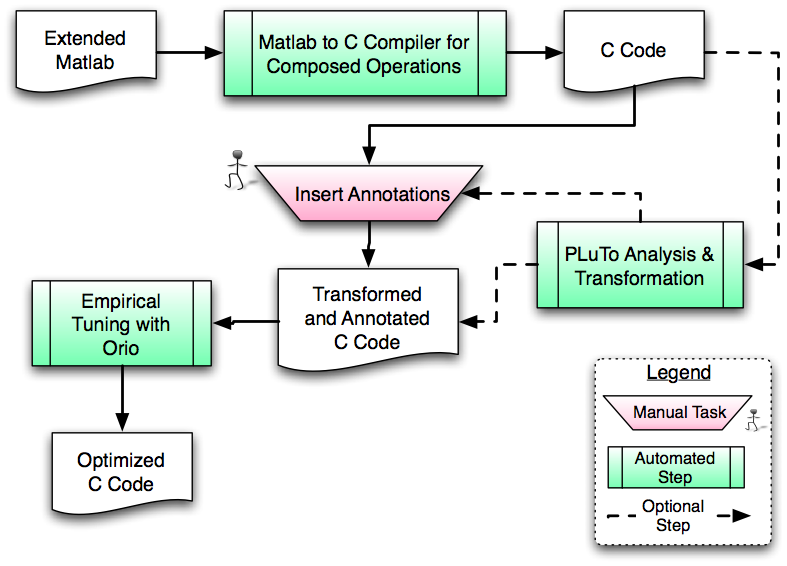
\includegraphics[width=.7\textwidth]{figures/process.png}

\caption{Overview of the code generation and tuning process, optional steps are indicated with dashed arrows.}
\label{fig:process}
\end{figure}
To generate highly optimized code from a MATLAB prototype of the composed BLAS operation, we follow a three-step approach, illustrated in Figure~\ref{fig:process}.  To begin, we have developed a compiler that converts a MATLAB script into simple C code.
%~\cite{Siek}. 
After generating the C code from the high-level MATLAB prototype, we (optionally) use the source-to-source automatic parallelization tool PLuTo\cite{Pluto} %developed at Ohio State University
to optimize for coarse-grained parallelism and locality simultaneously. Using the results of the PLuTo analysis, we insert annotations into the C code, which are then processed by our extensible annotation system Orio to generate many tuned versions of the same operation using different optimization parameters. Orio then performs an empirical search to select the best among the multiple optimized code variants.

%Probably need some words about WHY this multipronged approach is a good idea.

In the remainder of this section we describe each of the tools developed by the authors of this paper, namely the MATLAB to C compiler and the Orio empirical tuning tool.

\subsection{A MATLAB Compiler}
\label{sec:matlab}

In this section we describe the design and operation of the MATLAB to C compiler we have developed.    Figure~\ref{fig:compiler} gives an overview of the compilation process. The MATLAB kernel specification is parsed into a high-level intermediate representation in the form of a dataflow graph.  This dataflow graph is then iteratively processed until all of the implementation choices have been made.  The compilation process consists of three phases: analysis, lowering, and optimization, which are together iterated until all of the implementation decisions have been made.  The graph is then translated into C code.

\begin{figure}[htbp]
\centering
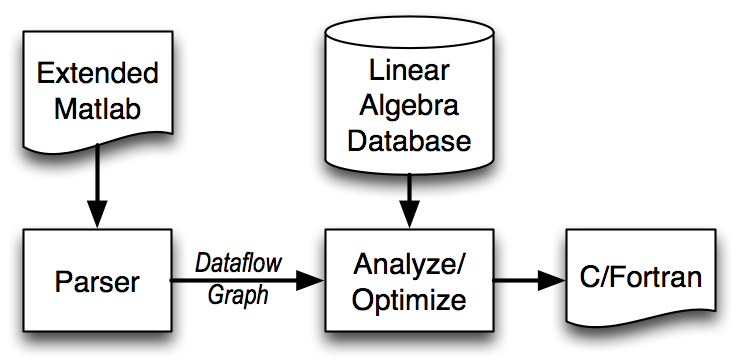
\includegraphics[width=.7\textwidth]{figures/compile.png}

\caption{Overview of the MATLAB compiler.}
\label{fig:compiler}
\end{figure}

\subsubsection{The Dataflow Graph}

An example dataflow graph for the GEMVER kernel, defined below, is given in figure~\ref{fig:gemver-dataflow}.
\begin{align*}
  A &\gets A + u_1 v_1^T + u_2 v_2^T \\[-0.5ex]
  x &\gets \beta A^T y + z \\[-0.5ex]
  w &\gets \alpha A x
\end{align*}
Each node represents a parameter of the kernel or an operation.  The arrows indicate the flow of data. At first the graph specifies what operations are to be performed but does not contain any implementation details. The symbol $\times$ in the depicted graph stands variously for outer product, matrix-vector multiplication, and scalar-vector multiplication, and it does not yet specify, for example, whether the outer products compute a row or a column at a time of the result matrix.

\begin{figure}[htbp]
\centering
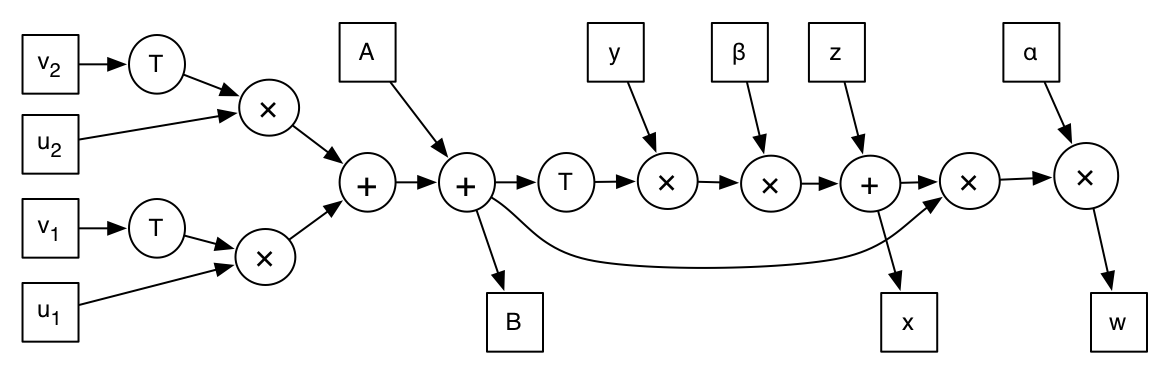
\includegraphics[width=.7\textwidth]{figures/gemver-dataflow.png}
 
\caption{Dataflow graph for the GEMVER kernel.}
\label{fig:gemver-dataflow}
\end{figure}

\subsubsection{Analyze the Dataflow Graph}

At the beginning of the analysis phase, each input and output node of the dataflow graph is labeled with its kind (scalar, vector, matrix, or unknown) and storage format (dense row-major, dense column-major, or unknown) according to the annotation given by the user.  During analysis, the kind and storage format are computed for the intermediate nodes and algorithms are assigned to operation nodes. The choice of algorithm and the determination of kinds of storage formats are interrelated so they must be computed together.  For example, the $\times$ symbol in the graph in Figure~\ref{fig:gemver-dataflow} having the inputs $u_1$ and $v_1^T$ can be implemented by iterating over rows first, or over columns first. The choice depends on how the result is used downstream in the dataflow graph.  In this case, the result is added to the outer product of $u_2$ and $v_2^T$, so we still could choose either option as long as we make the same choice for both outer products. Going one more step downstream, there is an addition with $A$, which was annotated in Figure~\ref{fig:gemver} to be column major. At this point it is clear that the outer-products should be computed in column-major order.

We do not hard code this knowledge of basic linear algebra in the compiler algorithm itself, but instead use a data-driven approach and store information regarding how to implement basic linear algebra in a separate database, which we refer to as the \emph{linear algebra database}.  This separation allows us to add new matrix formats, operations, and basic linear algebra algorithms without changes to the
compiler algorithm. 

The analysis algorithm makes implementation choices using the most-constrained first strategy (also called minimum remaining values)
from the artificial intelligence literature~\cite{Russell:2003mz}.
%This may need to be updated depending on how we decide to talk about the empirical search. -Jeremy 8/6/08 10:15 AM 
The compiler chooses the node with the fewest matching implementations (in the linear algebra database) and assigns a matching implementation to the node.  If there is more than one match, the prototype compiler picks the first.  Once we add backtracking we will push each alternative onto the stack to be explored later. Once the choice is made, the kind and storage format labels for the operation node itself and for the input nodes are updated with the labels specified in the linear algebra database for the chosen algorithm. The algorithm then goes on to find the next node with the fewest matching implementations and repeats.  In this phase, only the name of the algorithm is assigned to the operation node.  The details of the implementation are not specified until the refinement phase.


\subsection{Refine the Dataflow Graph}
\label{sec:refine}

The refinement phase resolves the implementation for each operation node in the graph into a subgraph defining the details of the chosen algorithm.  Each subgraph is an abstract representation of the loop that implements the given operation.  In each case, the subgraph has an iteration strategy that specifies how to traverse the elements of the matrix or vector.

Figure~\ref{fig:refine-mv-dot} shows two steps of refinement for a matrix-vector multiplication. The first step expands the matrix-vector multiplication according to the mv-dot algorithm: $(Ax)(i) = A(i,:)x$.  The refinement step replaces the $\times$ node with a subgraph that computes the inner product of a row of the matrix---the node labeled $(i,:)$---with the vector, storing the result in the $i$th element of the result vector---the node labeled $(i)$. The subgraph is labeled with $i=1\!:\!m$ indicating that the iteration strategy is to traverse the rows of the dense matrix.
%
The second pass of refinement introduces another subgraph to implement the inner products. The new subgraph iterates through each dense row, as indicated by the $j=1:n$ annotation. The sign $\Sigma$ indicates that the sum of all of the iterations is computed.


\begin{figure}[hbtp]
  \centering
  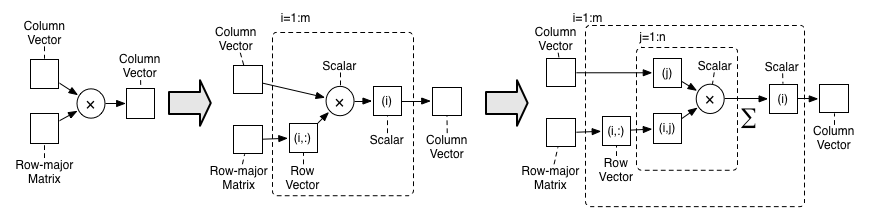
\includegraphics[width=\textwidth]{figures/refine-mv-dot.png}

  \caption{The refinement of a matrix-vector product to a set of inner products and the refinement of inner products to scalar multiplications and additions.}
  \label{fig:refine-mv-dot}
\end{figure}




\subsubsection{Optimize the Dataflow Graph}

In the optimization step, the dataflow graph is optimized by applying conditional graph rewrite rules.  One example rewrite rule is \emph{Merge Operand Sharing Subgraphs}: if two subgraphs share a common operand but do not depend on one another, and if the iteration strategies of the two subgraphs are compatible, then merge the subgraphs into a single subgraph.  This rule is responsible for fusing the loops of the two matrix-vector products in the GEMVER kernel.  Another example rule is \emph{Merge Dependent Subgraphs}: if one subgraph depends on another subgraph, and the iteration strategies of the two subgraphs are compatible, then merge them into a single subgraph.  This rule, for example, is responsible for fusing the loops of the two outer products in the GEMVER kernel.

The choice of which optimizations to apply to various parts of the graph depends on the characteristics of the kernel, the algorithm, the matrix order and kind, and architectural features.  The following is an instructive example: $y \gets A^T A (x + z + w)$.  Assume that the compiler has already merged the two vector additions into one subgraph, call it $S_1$, and the two matrix products into another subgraph, call it $S_2$. The question then is whether it is profitable to apply the Merge Dependent Subgraphs rule one more time to merge $S_1$ and $S_2$. If the three vectors plus a row of $A$ do not fit in cache, then the merger will not be profitable because it will cause each row of $A$ to fall out of cache before the row gets used a second time.  On the other hand, if all three vectors plus a row of $A$ do it in cache, then $S_1$ and $S_2$ should be merged.  In general, we need a way to search through the many different combinations of optimization choices and choose a combination that minimizes memory traffic.

\subsubsection{Translate the Dataflow Graph to C}

A graph that cannot be further refined has been reduced to a collection of subgraphs representing loops over scalar operations. The generator outputs a C loop for each subgraph.  A topological sort is performed to determine the order in which the loops and scalar operations within the loops appear in the output.
\subsection{Orio}
\label{sec:orio}

%~\cite{Norris:2007}
Orio is an empirical tuning tool that takes as input annotated C code and generates multiple tuned versions. Orio does not parse the application code; rather, it relies on annotations expressed as structured comments, which contain a simplified expression of the computation, as well as directives on what transformations to apply.

Figure~\ref{fig:orio} illustrates the tuning process using Orio. In the simplest case, Orio can be used to improve code performance by performing source-to-source transformations, such as loop unrolling and memory alignment optimizations. First, the input to Orio is C code, which contains syntactically structured comments that contain both the computation to be tuned, as well as various performance-tuning directives. Orio scans the annotated input code and extracts all annotated regions. Each annotated region is then passed to the code transformation modules for potential optimizations. The code generator then produces the final code incorporating the newly generated optimized C code corresponding to the annotation. The original C code is not parsed (only the annotation comments are processed) and is preserved in the new version. The user has the option of selecting either the original or the tuned code by using a compile-time macro.



\begin{figure}[htbp]
\centering
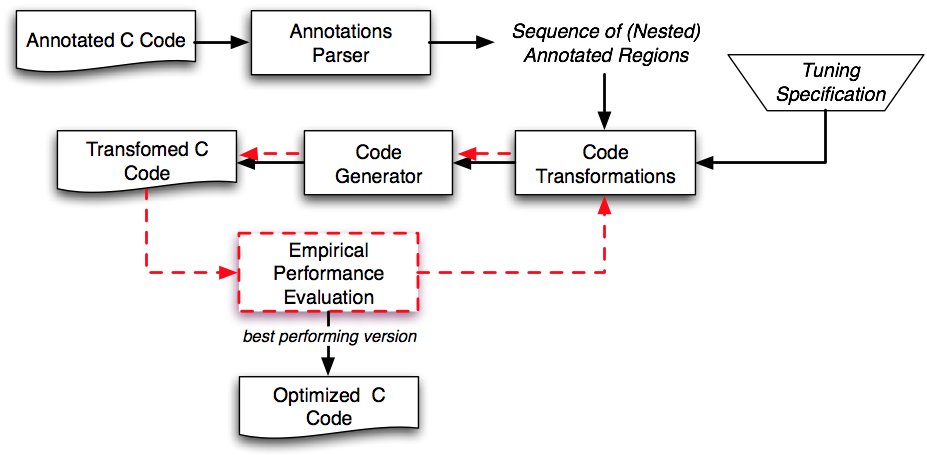
\includegraphics[width=.7\textwidth]{figures/orio.png}
\caption{Overview of the Orio empirical tuning process.}
\label{fig:orio}
\end{figure}


Orio can also be used as an automatic performance tuning tool. The system uses its code transformation modules and code generator to generate an optimized code version for each distinct combination of performance parameters. Then the optimized code versions are executed and their performance measured, which is subsequently compared to the performances of other previously tested code variants. After iteratively evaluating all code variants under consideration, the best-performing code is selected as the final output of Orio. The tuning specifications, written by users in the form of annotations (either embedded in the source code or in separate files), are parsed and used by Orio to guide the search and tuning process. These specifications include important information such as the used compilers, the search strategy, the program transformation parameters, the input data sizes, etc.

We use the VADD operation, $x = w + y + z$, as a simple example of the annotations and tuning specification used by Orio. Figure~\ref{fig:orio-example} shows the C code with annotation comments indicating that Orio should perform memory alignment and loop transformations. In addition to simple source transformation annotations in the example above, Orio supports a number of other transformations, including loop unroll and jam, composite optimizations, and architecture-specific directives (e.g., for generation of calls to SIMD intrinsics on the Blue Gene/P).

\begin{figure}[htp]
\centering
\begin{tabular}{cc}
\begin{minipage}[b]{.45\textwidth}
\scriptsize
\begin{verbatim}
void vadd(int n, double *y, double *x1,
               double *x2, double *x3)
{
    int i;

/*@ begin Align (x1[],x2[],x3[],y[]) @*/
/*@ begin Loop (
  transform Unroll(ufactor=20, parallelize=True)
    for (i=0; i < n; i++)
      y[i] = x1[i] + x2[i] + x3[i];
      ) @*/

    for (i=0; i < n ; i++)
        y[i] = x1[i] + x2[i] + x3[i];

/*@ end @*/
/*@ end @*/

}












\end{verbatim}
\end{minipage}
&
\begin{minipage}[b]{.45\textwidth}
\scriptsize
\begin{verbatim}
spec align_unroll {
 def build  
 { 
   arg build_command = 'mpixlc -O3 -qstrict -lm'; 
 } 
 def performance_counter  
 { 
   arg method = 'basic timer'; 
   arg repetitions = 10000;
 } 
 def performance_params 
 { 
   param UF[] = range(1,20);
 } 
 def input_params 
 { 
   param SIZE = @THESIZE@;
   decl int n = SIZE;
   decl double x1[n] = random;   
   decl double x2[n] = random;   
   decl double x3[n] = random;   
   decl double y[n] = 0;
 } 
 def search
 {
   arg algorithm = 'Exhaustive';
   arg time_limit = 20;
   arg run_command = 'cqsub -n 64 -t 10 -q short ';
   arg num_processes = 64;
 }
}
\end{verbatim}
\end{minipage}\\
\end{tabular}
\caption{Orio example: Annotated C source code (left) and a sample tuning specification for the Blue Gene/P (right).}
\label{fig:orio-example}
\end{figure}

On the right-hand side of Figure~\ref{fig:orio-example}, we show a separate tuning specification example, which contains the information required for creating complete executable tests and running them, including variable types, initializations (e.g., random), the search heuristic (in this case, exhaustive search is indicated, other options are random, simplex, and simulated annealing), and execution environment details. When parallel resources are available, Orio executes multiple variants in the same parallel job (the granularity is indicated by the \texttt{num\_processes} field in the search portion of the tuning specification. At present the tuning specification must be created manually. When Orio is used in conjunction with compiler tools, such as the MATLAB compiler described in this paper, it should eventually be possible to generate most of this tuning specification automatically.

\subsection{Search Space Exploration and Evaluation}
\label{sec:search}

% BN: moved to its own section since multiple tools deal with the search space problem.
The set of all possible combinations of implementation and optimization choices is called the search space~\cite{Kisuki:2000uq,Triantafyllis:2003uq,Cooper:2005kx}.  Although the dataflow graphs are quite small in our setting (usually less than 100 nodes), it is still important to prune the search space to avoid an exponential compilation time. Our prototype MATLAB compiler already performs some pruning: the optimization rewrite rules only apply under certain circumstances. 
%
% BN: commented out below since it's more future work
%However, as mentioned above we are sometimes overly aggressive in applying optimizations.
%To solve this problem we plan to use a combination of analytic methods and empirical methods~\cite{Chen:2007vn}.
%
Orio provides a number of different search heuristics to narrow the search space for near-optimal performance, including random, simplex, and simulated annealing searches. The search algorithm is one of the user-defined values in the Orio tuning specification.

\section{Experimental Results}
\label{sec:experiments}

In this section we present performance results for a number of composed BLAS operations. The experiment described in Section~\ref{sec:vadd} were performed on Blue Gene/P, while the remaining experiments described in this section were all performed on an Intel Xeon 2.80 GHz Intel(R) E5462 dual quad-core workstation with a 1600Mhz front-side bus and 16GB DDR2 FBDIMM RAM, running Ubuntu 8.04.

% Include peak numbers?

For the Xeon experiments, we used the Intel icc compiler (version 10.1) with the \texttt{-O3 -parallel} optimization flags. We generated and tested the following different implementations of each operation:
\begin{itemizer}
\item C from MATLAB: C code generated by the MATLAB compiler described in Section~\ref{sec:matlab}.
\item BLAS: A version implemented using multiple BLAS calls and linked with the default BLAS library available on Ubutnu 8.04.
\item Intel MKL: The same code as the BLAS version, but linked to the Intel MKL libraries.
\item ATLAS: The same code as the BLAS version, but linked to the ATLAS libraries tuned for this machine.
\item Orio (Seq.): The C code generated by the MATLAB compiler annotated with sequential-only optimization directives.
\item Orio (Par.) : The C code generated by the MATLAB compiler annotated with both sequential and parallel optimization directives (note that the code is the same as for Orio (Seq.), the only difference is the value of a parallelization parameter in the separate tuning specification). This version was compiled with the \texttt{-O3 -openmp} options.
\end{itemizer}

\subsection{VADD}
\label{sec:vadd}

The VADD operation computes the sum of three arrays, storing the result in a fourth: $x = w + y + z$.
We optimized the performance for the VADD operation on a Blue Gene/P
%at Argonne National Laboratory
using the IBM XLC compiler version 9.0. We measured the performance for two scenarios: using one core per processor and using all 4 cores on each processor. In the single-core case, the codes were compiled with the following options: \texttt{-O3 -qstrict -qarch=450d -qtune=450 -qhot -qsmp=noauto}. For the multicore case, the only difference in the compilation was that for the non-Orio versions, the \texttt{-qsmp=auto} option was used. The parallel Orio version differs from the sequential in that it contains parallelization directives, which result in the placement of OpenMP pragmas in the generated code.

\begin{figure}[htp]
\centering
\begin{tabular}{cc}
\begin{minipage}[b]{.25\textwidth}
\footnotesize
\begin{verbatim}
VADD
in
  w : vector,
  y : vector,
  z : vector
out
  x : vector
{
  x = w + y + z
}




\end{verbatim}
\end{minipage}
&
\begin{minipage}[b]{.6\textwidth}
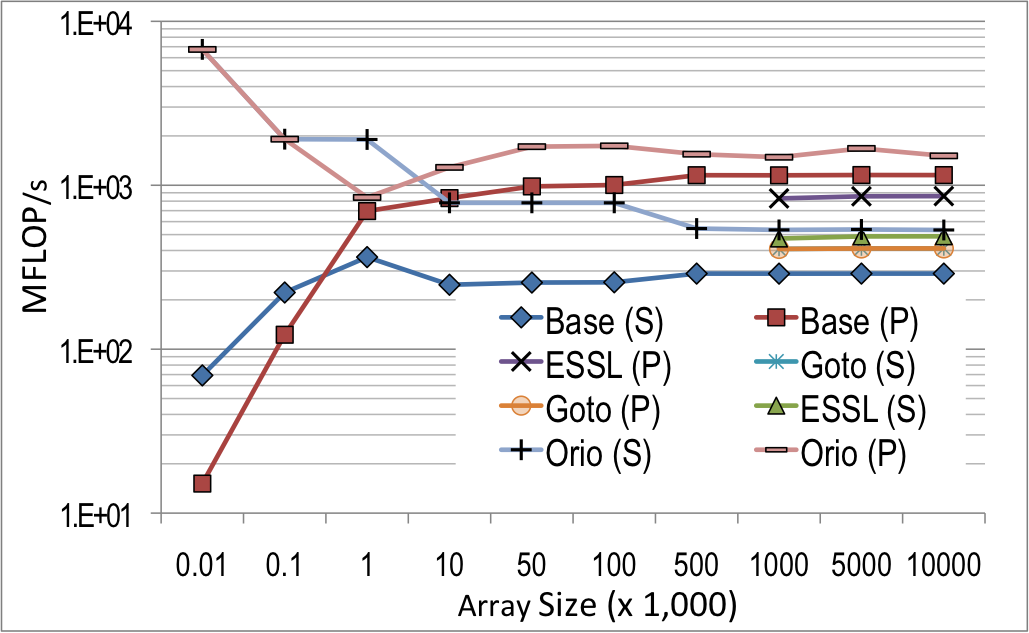
\includegraphics[width=\textwidth]{figures/vadd_bgp.png}
\end{minipage}\\
\end{tabular}
\caption{Annotated MATLAB code (left) and MFLOP/s (right) for the VADD operation using different code versions.}
\label{fig:vadd}
\end{figure}

The "Base" label designates the simple loop C implementation generated by the Matlab compiler, which was simply compiled with the options mentioned earlier and executed. We tested the performance of the IBM ESSL library and Goto BLAS for the two calls to \texttt{daxpy} used in the BLAS version of the code. Finally, we annotated the simple C loop version with memory alignment and loop unrolling directives, and then used Orio to select the best tuned version for the single-core and multicore scenarios. We observe that even for a very simple operation, such as the vector addition above, the compiler alone is unable to obtain the same level of performance as the empirically tuned versions. Furthermore, as expected, the BLAS performance was worse than that of the single loop implementation, however, selecting the correct compiler options was crucial for achieving good performance of the base version.

\subsection{ATAX}

The extended Matlab code for the ATAX operation, $y = A' * (A * x)$, and the corresponding performance results are shown in Figure~\ref{fig:atax}. The Orio-tuned version that incorporates PLuTo-generated loop fusion optimizations and Orio parallelization directives achieves the best performance for most problem sizes, outperforming the Intel MKL version by a factor of 2 to 5.7 and the compiler-optimized C version by a factor of 4 to 7. The optimizations performed by both Orio versions include scalar replacement, vectorization, and unroll and jam.



\begin{figure}[htp]
\centering
\begin{tabular}{cc}
\begin{minipage}[b]{.3\textwidth}
\footnotesize
\begin{verbatim}
ATAX
in
  A : row matrix,
  x : vector
out
  y : vector
{
  y = A' * (A * x)
}





\end{verbatim}
\end{minipage}
&
\begin{minipage}[b]{.6\textwidth}
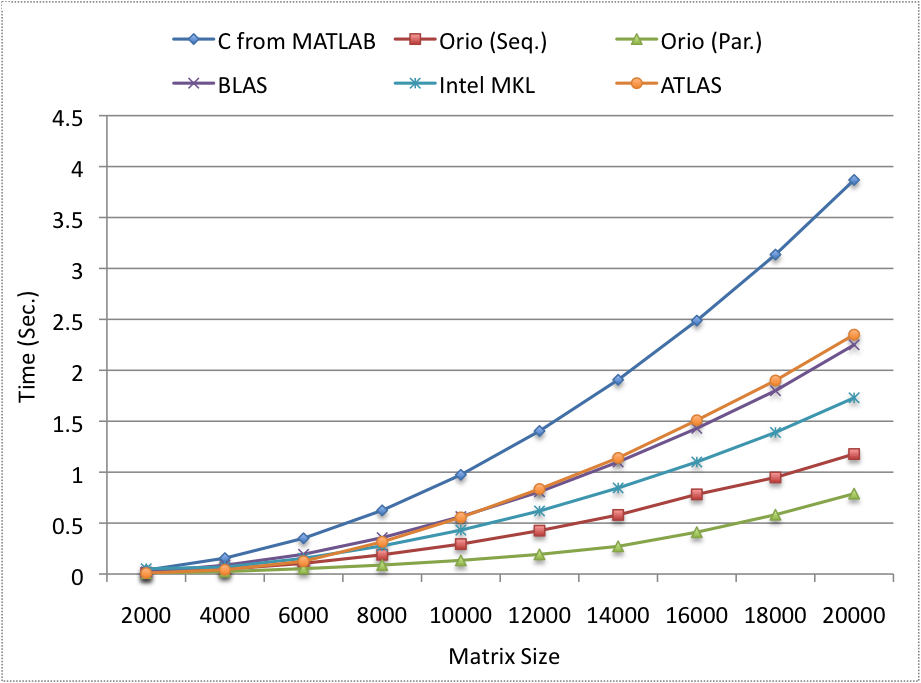
\includegraphics[width=\textwidth]{figures/atax.png}
\end{minipage}\\
\end{tabular}
\caption{Annotated MATLAB code (left) and wall-clock time in seconds (right) for the ATAX operation using different code versions.}
\label{fig:atax}
\end{figure}

\subsection{GEMVER}


The extended MATLAB code for the GEMVER operation and the corresponding performance results are shown in Figure~\ref{fig:gemver}. Here we used the same PLuTo and Orio optimizations as for the ATAX example and similarly the parallel Orio version achieves the best performance, although in this case the sequential Orio version performs almost as well suggesting that the compiler was not able to parallelize the code very effectively. For this operation, there are substantial performance differences between different BLAS versions, with the Intel MKL version achieving performance close to that of the simple compiler code.
\begin{figure}[htp]
\centering
\begin{tabular}{cc}
\begin{minipage}[b]{.3\textwidth}
\footnotesize
\begin{verbatim}
GEMVER
in
  A : column matrix,
  u1 : vector, u2 : vector,
  v1 : vector, v2 : vector,
  a : scalar, b : scalar,
  y : vector, z : vector
out
  B : column matrix,
  x : vector, w : vector
{
  B = A + u1 * v1'
           + u2 * v2'
  x = b * (B' * y) + z
  w = a * (B * x)
}
\end{verbatim}
\end{minipage}
&
\begin{minipage}[b]{.6\textwidth}
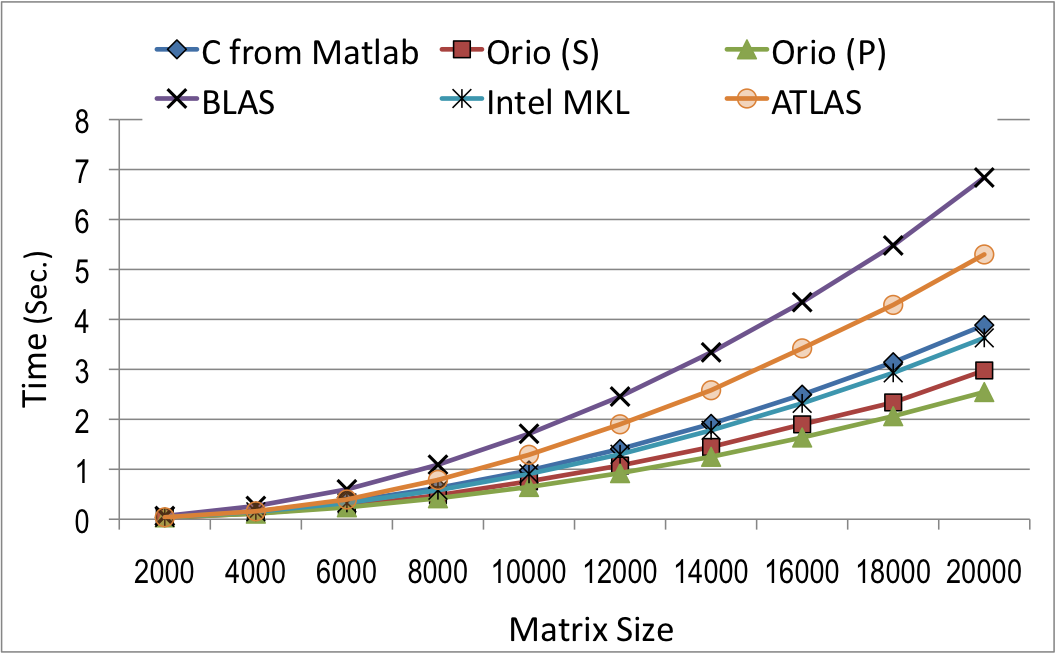
\includegraphics[width=\textwidth]{figures/gemver.png}
\end{minipage}\\
\end{tabular}
\caption{Annotated MATLAB code (left) and wall-clock time in seconds (right) for the GEMVER operation using different code versions.}
\label{fig:gemver}
\end{figure}

% Data (Dual quad-core Intel Xeon E5462, 16GB RAM)
%--- Sequential: seconds (dynamic arrays) ---
%cmatlab= [0.038, 0.157, 0.352, 0.626, 0.976, 1.406, 1.909, 2.494, 3.143, 3.886]
%orio= [0.029, 0.118, 0.263, 0.480, 0.759, 1.075, 1.447, 1.899, 2.338, 2.978]
%blas= [0.064, 0.265, 0.598, 1.091, 1.711, 2.456, 3.340, 4.345, 5.480, 6.840]
%mkl=  [0.073, 0.147, 0.331, 0.591, 0.923, 1.326, 1.803, 2.350, 2.975, 3.676]
%atlas=[0.039, 0.163, 0.401, 0.796, 1.225, 1.916, 2.582, 3.381, 4.210, 4.756]
%
%--- Parallel: seconds (dynamic arrays) --- N=10,000, cores=1-8
%cmatlab= [0.976, 0.976, 0.976, 0.976, 0.976, 0.976, 0.975, 0.976]
%orio= [0.754, 0.738, 0.666, 0.649, 0.664, 0.664, 0.647, 0.668]


\subsection{GESUMMV}


The extended Matlab code for the GESUMMV operation, $y = a * (A * x) + b * (B * x)$,
and the corresponding performance results are shown in Figure~\ref{fig:gesummv}. Unlike all the other operations we tested, the best performing version is the ATLAS one, which substantially outperforms all the alternatives. The next best performance is exhibited by the parallel Orio version. This result motivates the development of transformations that enable the generation of code with calls to existing optimizing libraries in addition to the low-level loop transformations targeted by the current tools (PLuTo and Orio).


\begin{figure}[htp]
\centering
\begin{tabular}{cc}
\begin{minipage}[b]{.3\textwidth}
\footnotesize
\begin{verbatim}
GESUMMV
in
  A : row matrix,
  B : row matrix,
  x : vector,
  a : scalar,
  b : scalar
out
  y : vector
{
  y = a * (A * x)
       + b * (B * x)
}



\end{verbatim}
\end{minipage}
&
\begin{minipage}[b]{.6\textwidth}
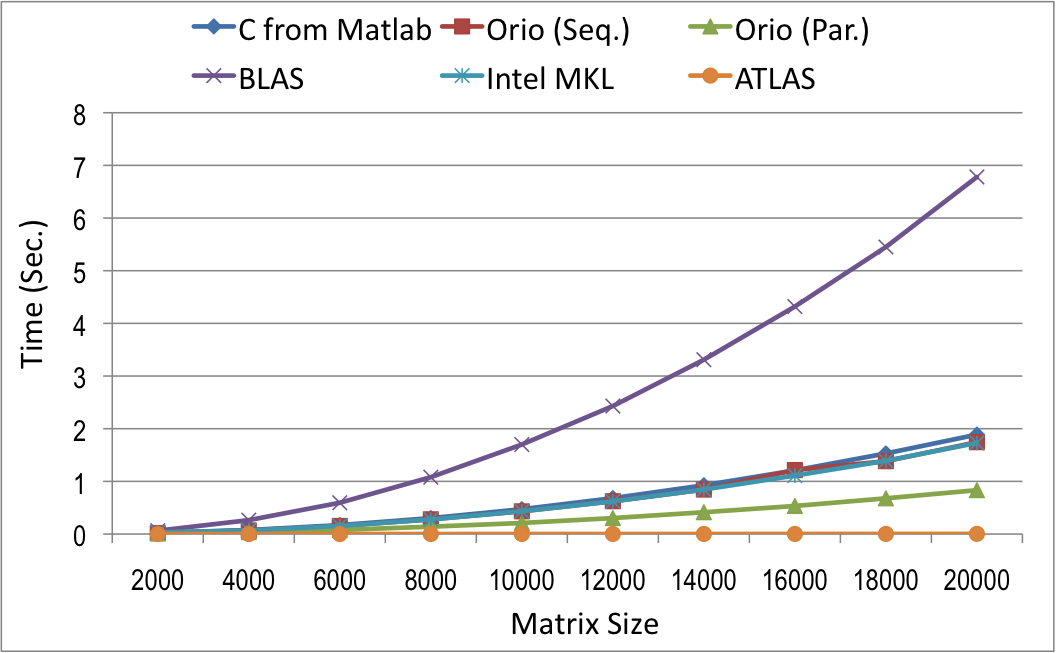
\includegraphics[width=\textwidth]{figures/gesummv.png}
\end{minipage}\\
\end{tabular}
\caption{Annotated MATLAB code (left) and wall-clock time in seconds (right) for the GESUMMV operation using different code versions.}
\label{fig:gesummv}
\end{figure}


% BN: ATLAS's dgemv is annihilating everything else, even though it's called twice... wow.
% I did check the result and it was correct, i'm still somewhat baffled
% The Time and MFLOPS data for the above are (with icc):
% (Dual quad-core Intel Xeon E5462, 16GB RAM)
% ops = (4*N*N+3*N)
% --- Parallel: seconds (dynamic arrays) ---
%matlabc= [0.019, 0.075, 0.170, 0.301, 0.471, 0.678, 0.923, 1.205, 1.529, 1.887]
%blas= [0.00006, 0.00018, 0.00039, 0.00060, 0.00090, 0.00126, 0.00168, 0.00216, 0.00270, 0.00330]
%orio= [0.013, 0.035, 0.076, 0.133, 0.210, 0.300, 0.410, 0.533, 0.676, 0.831]
%--- Parallel: Mflops/sec (dynamic arrays) ---
%matlabc= [846.565, 848.425, 849.028, 849.503, 849.690, 849.968, 849.605, 849.946, 847.893, 848.023]
%blas= [271288.136, 347891.304, 367392.857, 421785.832, 480228.091, 497440.415, 508787.800, 516153.226, 524930.741, 530172.300]
%orio= [1231.989, 1846.163, 1885.595, 1918.746, 1907.976, 1920.818, 1910.867, 1920.502, 1915.970, 1924.623]
%
% and gcc behaves similarly, so it's not icc being smart and detecting 2 calls to dgemv
% time: blas= [0.000, 0.000, 0.000, 0.001, 0.001, 0.001, 0.002, 0.002, 0.003, 0.003]
% mflops: blas= [254063.492, 346010.811, 393491.803, 421785.832, 439593.407, 453214.792, 463108.092, 470394.120, 462381.020, 469088.244]



\subsection{BiCG Kernel}

% No pluto
The extended Matlab code for the BiCG Kernel operation,$q = A * p$, $s = A' * r$,
and the corresponding performance results are shown in Figure~\ref{fig:gesummv}. For this operation, the PLuTo analysis did not result in performance improvement, thus we are showing the results obtained only through Orio transformations, which included vectorization, scalar replacement, and unroll and jam. Again the best performance was exhibited by the parallel Orio version, while all the BLAS versions performed worse than the compiler-optimized C loop version.


\begin{figure}[htp]
\centering
\begin{tabular}{cc}
\begin{minipage}[b]{.3\textwidth}
\footnotesize
\begin{verbatim}
BICG
in
  A : column matrix,
  p : vector, r : vector
out
  q : vector, s : vector
{
  q = A * p
  s = A' * r
}



\end{verbatim}
\end{minipage}
&
\begin{minipage}[b]{.6\textwidth}
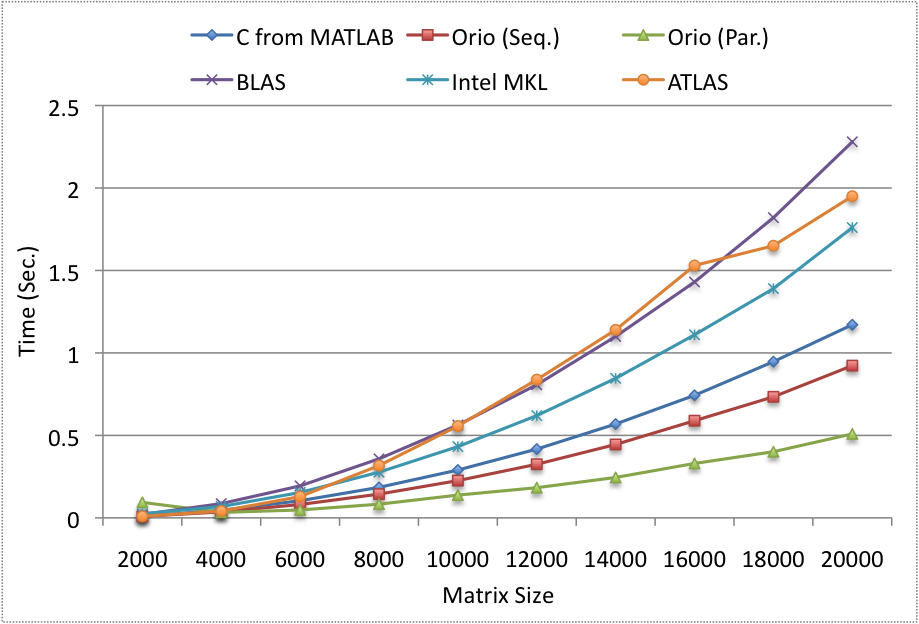
\includegraphics[width=\textwidth]{figures/bicgkernel.png}
\end{minipage}\\
\end{tabular}
\caption{Annotated MATLAB code (left) and wall-clock time in seconds (right) for the BiCG kernel operation using different code versions.}
\label{fig:bicgkernel}
\end{figure}

\section{Conclusions and Future Work}

We have described an approach to generating tuned linear algebra libraries from high-level annotated MATLAB code that involves a suite of tools to (1) translate the MATLAB code to C, (2) analyze the resulting loops and identify locatility and parallelism-enhancing optimizations using PLuTo, and (3) annotate the resulting C code with syntactic performance directives and use Orio to generate multiple optimized versions and empirically select the one with the best performance. Preliminary results from experiments with several composed BLAS operations show that in almost all cases, the optimized code generated by this suite of tools significantly outperforms the versions using tuned BLAS and aggressive compiler optimizations.

The positive initial results from our approach to generating tuned linear algebra routines motivate several future lines of investigation. At present there are a number of manual steps involved in obtaining a compiled tuned linear algebra library from the high-level extended MATLAB descriptions. We will work on interfacing our separately developed tools more closely and automating their interactions. This would enable application developers to easily produce custom linear algebra libraries tuned for specific architectures. We will also investigate extending the supported functionality of our MATLAB compiler beyond composed BLAS operations, thus benefiting a wider spectrum of applications.

Orio is growing in a number of directions. While it automates much of the tuning process, a number of steps still require nontrivial manual input. Orio's modular design allows new transformations to be added easily, which presents many opportunities for expanding the existing set of optimizations with new ones implemented from scratch or through interfaces to other tools, as we have successfully done with PLuTo. We are also working on generating code that contains special cases for different input parameter values since in many cases different optimizations are optimal for different input sizes.  We will also continue developing the parallel empirical search infrastructure; it is clear that more feedback between the MATLAB compiler and Orio will result in automation of the performance directive annotation process and a much more effective exploration of the search space. We plan to use a fast analytic cost function in the MATLAB compiler implementation to prune out regions of the search space that will not produce competitive implementations. The cost function is based on a model of the computer architecture, but does not necessarily account for all the details. Once the search space is narrowed, we will use the Orio empirical testing results with representative data sets to determine the exact performance of the alternatives and choose the best one.

Finally, while Orio currently generates various loop transformations, it does not generate calls to existing library implementations. For this paper, we implemented the BLAS versions of all operations manually. Our past success with identifying Blue Gene/L intrinsics from expression graphs motivate further research on identifying BLAS and other established library operations from the expression graphs of the MATLAB code.

%\singlespacing
%% or stuff it in a footnote
%\section*{Acknowledgments}
%This work was supported by the Mathematical, Information, and
%Computational Sciences Division subprogram of the Office of Advanced
%Scientific Computing Research, Office of Science, U.S. Dept. of Energy,
%under Contract DE-AC02-06CH11357. 
%TODO: need Colorado and Ohio acknowledgments

\bibliographystyle{splncs}
\bibliography{paper}

%\vfill
%\begin{flushright}
%\scriptsize
%\framebox{\parbox{2.4in}{The submitted manuscript has been created by
%UChicago Argonne, LLC, Operator of Argonne National Laboratory
%("Argonne").  Argonne, a U.S. Department of Energy Office
%of Science laboratory, is operated under Contract No.
%DE-AC02-06CH11357.  The U.S. Government retains for itself, and
%others acting on its behalf, a paid-up, nonexclusive, irrevocable
%worldwide license in said article to reproduce, prepare derivative works,
%distribute copies to the public, and perform publicly and display
%publicly, by or on behalf of the Government.}}
%\normalsize
%\end{flushright}

\end{document}



% Current bibtex warnings:
This is BibTeX, Version 0.99c (Web2C 7.5.4)
The top-level auxiliary file: paper.aux
The style file: siam.bst
Database file #1: paper.bib
Warning--can't use both volume and number fields in TCE
(There was 1 warning)


% Put bibtex here only if you do not have access to the subversion repository, otherwise insert them into paper.bib


